%=======================================================================
%  Unsupervised Crop Stress Detection from Sentinel-2 Time Series
%  IEEE conference format (IEEEtran). Compile with pdflatex:
%      pdflatex main && bibtex main && pdflatex main && pdflatex main
%  Overleaf: upload main.tex, refs.bib and figures/, compiler pdfLaTeX.
%
%  Every number in this file comes from
%      crop_stress/outputs/study/results.json
%  via outputs/REPORT.md. Do not edit numbers here by hand — regenerate
%  the study and copy them across, or the paper and the code will drift.
%=======================================================================
\documentclass[conference]{IEEEtran}
\IEEEoverridecommandlockouts

\usepackage{cite}
\usepackage{amsmath,amssymb}
\usepackage{graphicx}
\usepackage{booktabs}
\usepackage{url}
% stfloats lets a full-width figure* be set at the BOTTOM of a page in
% twocolumn mode. Without it a figure* can only go at the top, which halves the
% available slots and is what pushed the wide float into the bibliography.
\usepackage{stfloats}
\usepackage[hidelinks]{hyperref}

\graphicspath{{figures/}}
\newcommand{\tabfont}{\footnotesize}

% Give LaTeX more room to place floats before it gives up and defers them.
% IEEEtran's defaults are tight for a paper with this many exhibits.
\renewcommand{\topfraction}{0.9}
\renewcommand{\bottomfraction}{0.7}
\renewcommand{\textfraction}{0.1}
\renewcommand{\floatpagefraction}{0.75}
\setcounter{topnumber}{3}
\setcounter{bottomnumber}{2}
\setcounter{totalnumber}{4}

\begin{document}

%=======================================================================
\title{Unsupervised Crop Stress Detection from\\
Sentinel-2 Time Series: Ensemble Dilution and the\\
Primacy of Threshold Calibration}

\author{\IEEEauthorblockN{[Author Name]}
\IEEEauthorblockA{[Department]\\
[Institution]\\
[City, Country]\\
prakharpaawan@gmail.com}
}

\maketitle

%=======================================================================
\begin{abstract}
Crop stress detection from satellite imagery is limited by the cost of
ground-truth labels: an agronomist must visit a field to say whether it is
diseased, drought-stricken or healthy. We present a fully unsupervised
tile-level stress detector for Sentinel-2 time series that uses no labels at
any stage, evaluated on 3{,}328 georeferenced 480\,m tiles in Lombardy, Italy across
25 cloud-screened passes of the 2019 season. Detection performance is measured
by injecting synthetic stress into clean data and measuring recovery, under a
protocol in which the detector is fitted on one set of tiles, every decision
threshold is calibrated on clean pre-injection scores, hyperparameters are
selected on a second set of tiles, and all reported numbers come from a third,
untouched set. We report two findings and one correction. First, a negative
result: score-level ensembling of Isolation Forest, Local Outlier Factor (LOF)
and an autoencoder --- the architecture this system was built around --- reaches
F1 $0.354$, while standalone LOF reaches $0.844$ under an identical protocol.
The ensembles do not produce wrong alarms; they stop producing alarms at all,
with recall falling from $0.814$ to $0.230$. Second, and more consequential in
practice, \emph{where} the threshold is computed matters more than \emph{which}
detector is used: calibrating each tile's threshold on clean scores rather than
on the batch containing the anomalies raises F1 from $0.693$ to $0.844$ with the
detector untouched, an improvement of $+0.151$ (95\%~CI $[+0.142, +0.159]$,
paired permutation $p < 5 \times 10^{-4}$). Fitting an extreme-value tail to each tile's
clean scores attains the same accuracy while replacing an arbitrary percentile
with a stated false-alarm risk. Third, we correct a claim from our own earlier
work: an apparent collapse in performance under held-out evaluation, measured by
comparing two separate implementations, does not survive a controlled test.
Holding everything but the protocol fixed, held-out evaluation costs $0.021$~F1.
We report throughout that the recommended operating point is \emph{worse} than
the one it replaces on events below roughly 30\% severity, which is where early
warning has the most value.
\end{abstract}

\begin{IEEEkeywords}
anomaly detection, precision agriculture, Sentinel-2, remote sensing, local
outlier factor, extreme value theory, unsupervised learning, negative results
\end{IEEEkeywords}

%=======================================================================
\section{Introduction}

Crop stress --- from disease, drought, nutrient deficiency or pest pressure ---
depresses yield before it is obvious to an observer standing in the field.
Detecting it early and at scale is one of the clearest applications of free
optical satellite imagery. Sentinel-2 supplies multispectral acquisitions at
$10$--$20$\,m resolution on a five-day revisit at no cost \cite{drusch2012},
enough to track the seasonal trajectory of an individual parcel.

The obstacle is labels, not imagery. Supervised stress detection needs a record
of which field was stressed, when, and how badly. Producing it means field
visits by trained agronomists: expensive, slow, and unable to scale to the tens
of thousands of parcels in one administrative region. Published supervised
results are therefore usually confined to small, intensively surveyed study
areas \cite{weiss2020,mahlein2016}.

This paper takes the unsupervised route. We treat stress as an anomaly in a
tile's own temporal behaviour and ask which observations depart from the
distribution of normal tile-seasons. No label enters at any stage. To obtain
precision and recall without ground truth we inject synthetic stress into clean
data and measure recovery, a standard device in the unsupervised
outlier-detection literature \cite{campos2016,emmott2013}.

We set out to build a hybrid ensemble, on the common intuition that combining
detectors with different inductive biases is more robust than any one of them.
A systematic ablation showed the opposite. Pursuing that result, rather than
tuning past it, produced the rest of this paper.

\textbf{Contributions.}
\begin{enumerate}
\item \emph{A negative result on ensembling.} Score-level fusion of Isolation
Forest, LOF and an autoencoder degrades F1 from $0.844$ to $0.354$ relative to
standalone LOF under an identical protocol (Section~\ref{sec:models}). We
identify the mechanism --- the ensembles lose recall, not precision --- and
report it in place of the architecture we intended to publish.
\item \emph{Threshold placement dominates detector choice.} Calibrating each
tile's threshold on clean scores instead of on the batch containing the
anomalies raises F1 by $0.151$ with the detector unchanged
(Section~\ref{sec:threshold}). We give the mechanism, and show that an
extreme-value tail attains the same accuracy with an interpretable risk
parameter in place of a percentile.
\item \emph{A correction to our own earlier claim.} A large apparent cost of
held-out evaluation, obtained by comparing two implementations, does not
survive a controlled test: the true cost is $0.021$~F1
(Section~\ref{sec:protocol}).
\item An evaluation protocol in which no reported number is selected on, and an
explicit account of where the recommended configuration is worse than the one
it replaces (Section~\ref{sec:limits}).
\end{enumerate}

%=======================================================================
\section{Related Work}

\textbf{Vegetation indices.} NDVI \cite{rouse1974} remains the default proxy for
canopy vigour but saturates over dense canopy and is contaminated by soil
background when the canopy is sparse. We use MSAVI \cite{qi1994}, which replaces
the fixed soil factor of SAVI \cite{huete1988} with a self-adjusting term,
because the early-season signal in our region is dominated by bare soil.
Red-edge indices such as NDRE respond to chlorophyll before the visible bands do
\cite{gitelson1994}, and the SWIR moisture index NDMI responds to canopy water
content \cite{gao1996}; Section~\ref{sec:forward} returns to these.

\textbf{Satellite time-series change detection.} BFAST \cite{verbesselt2010}
decomposes an index series into trend, seasonal and remainder components and
locates breakpoints; CCDC \cite{zhu2014} fits harmonic models and flags
departures. Both target land-cover change --- deforestation, urban expansion ---
where change is permanent and structural. Crop stress is transient, partial and
superimposed on a strong phenological signal that is itself changing rapidly.
The family is reviewed in \cite{zhu2017}.

\textbf{Unsupervised anomaly detection.} We evaluate three families
\cite{chandola2009,ruff2021}. Isolation Forest \cite{liu2008} isolates points by
random axis-aligned splits, which works when anomalies are globally extreme.
LOF \cite{breunig2000} compares a point's local reachability density with that
of its neighbours, detecting points unusual \emph{relative to their local
neighbourhood} even when unremarkable globally. Autoencoders score by
reconstruction error under a bottleneck trained on normal data
\cite{sakurada2014}. A large benchmark study \cite{han2022} found no detector
dominant across datasets, with LOF specifically favoured for local anomalies ---
which our results bear out.

\textbf{Thresholding.} Most unsupervised pipelines convert a score to a decision
with a percentile, chosen by hand. Siffer et al.\ \cite{siffer2017} instead fit
a Generalised Pareto tail to the extremes of a score stream and invert it for a
target false-alarm risk, following the peaks-over-threshold result of Pickands
\cite{pickands1975} and Balkema and de Haan \cite{balkema1974}. We adopt this,
and Section~\ref{sec:threshold} argues that thresholding deserves more attention
than it usually receives in this literature.

\textbf{Evaluating unsupervised detectors.} Campos et al.\ \cite{campos2016}
showed measured performance in unsupervised outlier detection is extremely
sensitive to preparation and normalisation choices, and that cross-paper
comparisons are frequently comparisons of protocol. Section~\ref{sec:protocol}
tests that effect on our own system and finds it real but far smaller than an
uncontrolled comparison suggested.

%=======================================================================
\section{Data and Method}
\label{sec:method}

\begin{figure}[!t]
\centering
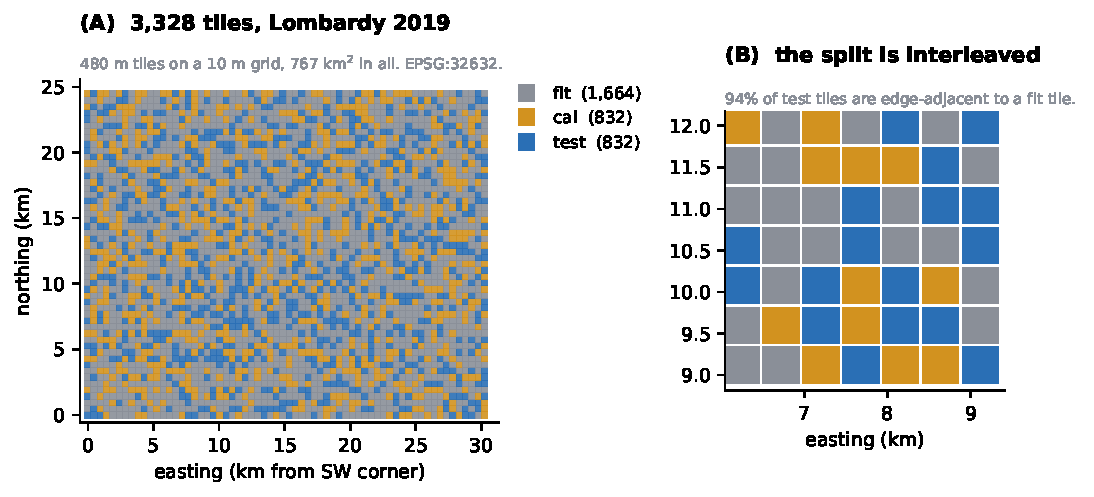
\includegraphics[width=\columnwidth]{study_area.pdf}
\caption{The study area. \textbf{(A)} All $3{,}328$ tiles in their true
positions: a near-contiguous $30.2 \times 24.5$\,km block of $480$\,m tiles,
$767$\,km$^2$ in all, coloured by the split each is assigned to.
\textbf{(B)} A seven-tile detail. The split is drawn at random over tile
identifiers, so held-out tiles are interleaved with the tiles the detector is
fitted on rather than separated into a distinct region; Section~\ref{sec:forward}
states what that costs.}
\label{fig:studyarea}
\end{figure}

\begin{figure}[!t]
\centering
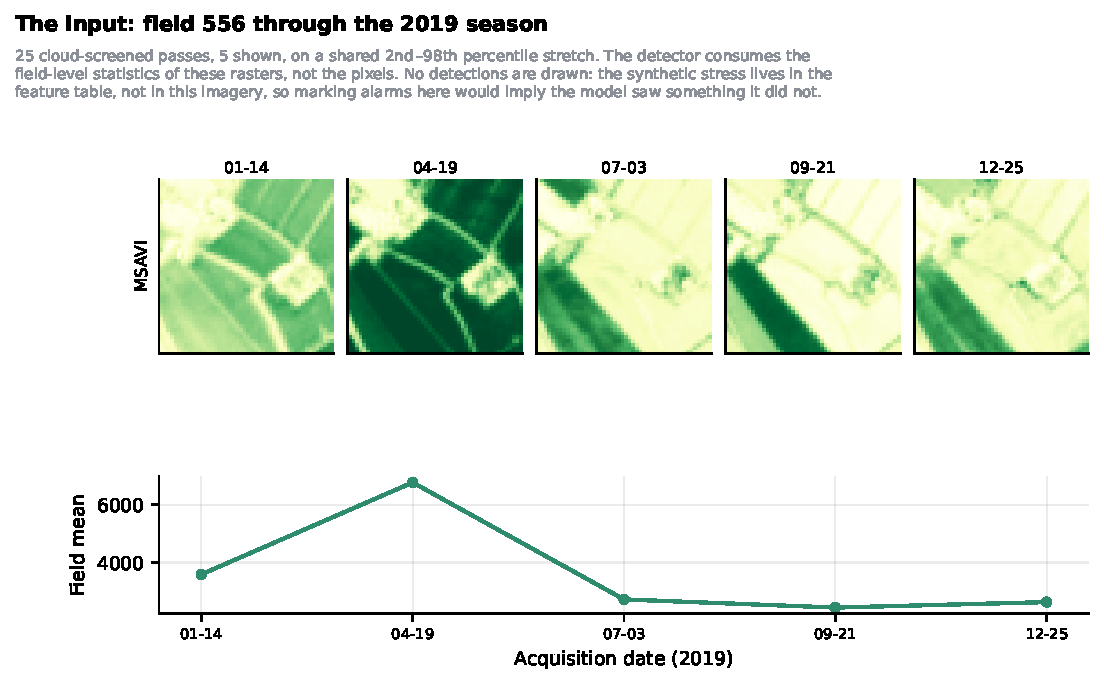
\includegraphics[width=\columnwidth]{imagery.pdf}
\caption{The input: one $480$\,m tile through 2019, on a shared
2nd--98th percentile stretch, with the tile-mean trajectory beneath. Several
cropped fields are visible within the tile, which is the granularity the method
works at. The detector consumes tile-level statistics of these rasters, not the
pixels. No detections are drawn: the synthetic stress used for evaluation lives
in the feature table rather than in this imagery.}
\label{fig:imagery}
\end{figure}

The study region is Lombardy, northern Italy --- an intensively cultivated plain
of maize, rice, wheat and forage. The archive holds Sentinel-2 acquisitions over
$3{,}328$ sites for 2016--2019; this study uses 2019.

\textbf{The unit of analysis is a fixed tile, not a digitised parcel.} Each site
is a $48 \times 48$ pixel square at $10$\,m resolution --- $480$\,m on a side,
$23$\,ha --- on a regular grid, and every pixel in it is retained. In a plain
farmed at this intensity a tile of that size will usually span more than one
cropped field (visible in Fig.~\ref{fig:imagery}), so the detector's unit is a
neighbourhood rather than a management unit. We use \emph{tile} throughout in
preference to \emph{parcel}. The tiles cover a near-contiguous
$30.2 \times 24.5$\,km block, $767$\,km$^2$ in total, in UTM zone 32N
(EPSG:32632); Fig.~\ref{fig:studyarea} maps them.

\textbf{Screening.} Optical imagery over an agricultural plain is heavily
cloud-affected, and a cloud-covered acquisition produces exactly the signature a
stress detector looks for. Acquisitions are rejected on four criteria: a minimum
intensity standard deviation (a uniform raster is cloud or fill), a minimum
valid-pixel ratio of $0.7$, a minimum unique-value ratio of $0.05$, and a
minimum spatial gradient magnitude (a real field has texture; a cloud top does
not). We then select $25$ passes per tile at least $10$ days apart, spanning the
2019 calendar year, giving $3{,}328 \times 25 = 83{,}200$ tile-observations.
Because screening rejects any acquisition below a $0.7$ valid-pixel ratio, every
retained raster is a full square of valid pixels --- a fact we return to below.

\textbf{Features.} For each tile and pass we mask nodata, clip to the 1st and
99th percentiles --- removing specular glare without disturbing the bulk of the
distribution --- and compute descriptive statistics over the tile. These are
augmented with temporal context computed within each tile: rolling median and
standard deviation over three acquisitions, first difference and percent change,
deviation from the dataset median, and a Savitzky--Golay smoothed
\cite{savitzky1964} tile median. Smoothing matters more than it appears to: a
single cloud-shadowed pass produces a one-observation cliff indistinguishable
from a crop dying, and local polynomial fitting restores a biologically
plausible curve while preserving genuine multi-pass declines --- the rationale
that motivates its use in NDVI reconstruction \cite{chen2004}. This yields $16$
feature columns per tile-observation, of which $15$ vary.

Aggregating to the tile is deliberate, though the unit is coarser than a
management decision. It averages away the per-pixel noise that dominates
$10$\,m optical data (Fig.~\ref{fig:imagery}) and yields one decision per tile
per pass, which is a tractable inspection queue at regional scale. The cost is
twofold: the system says \emph{this tile, this week} rather than \emph{this
corner of this field}, and because a $23$\,ha tile may hold more than one crop,
an alarm localises a neighbourhood to visit rather than a field to treat.

\textbf{Detectors.} Three are fitted on standardised clean features: Isolation
Forest \cite{liu2008} with $100$ estimators; LOF \cite{breunig2000} in novelty
mode with $k=10$; and a $16\!\to\!32\!\to\!4\!\to\!32\!\to\!16$ autoencoder with
dropout $0.2$, trained $200$ epochs with Adam at $10^{-3}$, scored by
reconstruction error. A \textbf{hybrid} min--max normalises the three scores and
combines them by a weighted sum, at equal weights
($0.33, 0.33, 0.34$). Implementations are scikit-learn
\cite{pedregosa2011} and PyTorch \cite{paszke2019}.

\textbf{Three inert components,} recorded because they are easy to claim as
method when they are not. A PCA retaining $95\%$ of variance is fitted by the
pipeline but consumed by nothing; it is not part of the method and we do not
claim it. The \texttt{contamination} parameter of Isolation Forest and LOF has
no effect on any result here: it only shifts the decision offset used by the
library's \texttt{predict()} path, while we score with raw sample scores and
apply our own threshold, and a constant offset cannot change a percentile
ranking. This is an advantage rather than an oversight --- the true
contamination rate is unknown in practice, and the method does not need it.
Third, one of the $16$ feature columns is constant. Screening admits only
acquisitions above a $0.7$ valid-pixel ratio and the retained rasters are full
squares, so \texttt{valid\_pixel\_ratio} is $1.0$ for all $83{,}200$
observations; after standardisation it contributes nothing, and the effective
feature count is $15$. We report the ablations against the $16$-column set as
run, since removing a zero-variance column cannot change a distance-based score.

\subsection{Decision rule}

\begin{figure}[!t]
\centering
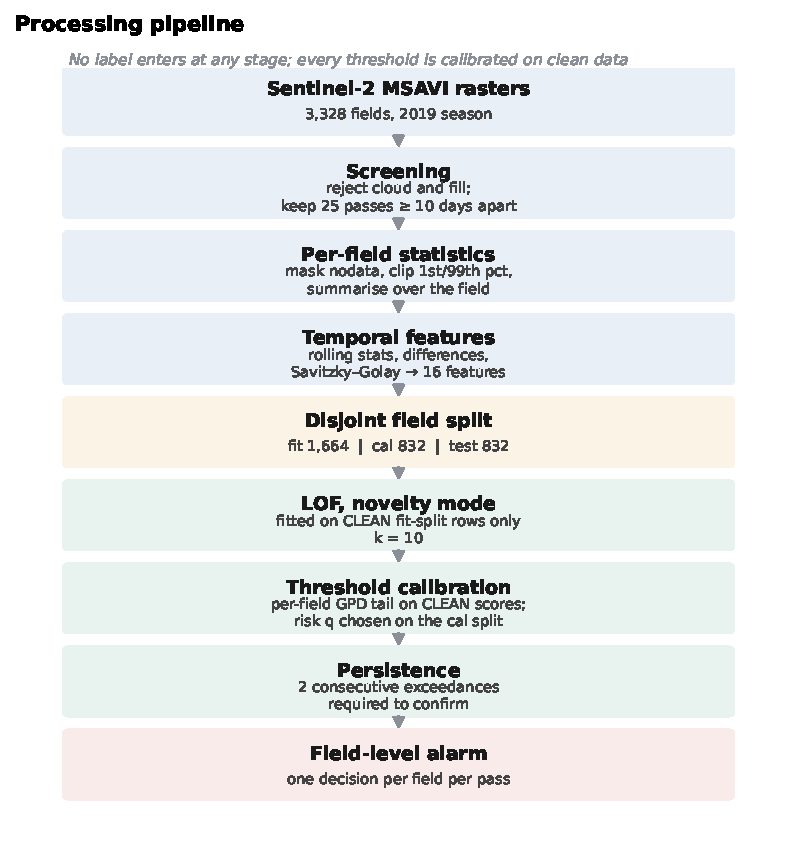
\includegraphics[width=0.84\columnwidth]{pipeline.pdf}
\caption{Processing pipeline. No label enters at any stage, and every threshold
is calibrated on clean data. The three-way tile split is the device that makes
the reported numbers safe to quote: hyperparameters are chosen on the
calibration tiles and nothing is selected on the test tiles.}
\label{fig:pipeline}
\end{figure}

\begin{figure}[!t]
\centering
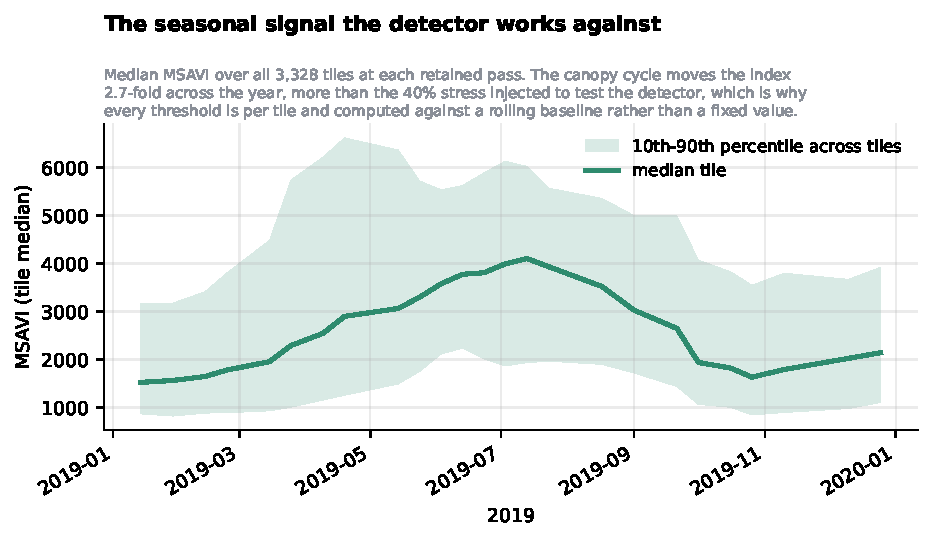
\includegraphics[width=\columnwidth]{phenology.pdf}
\caption{Median MSAVI across all $3{,}328$ tiles at each retained pass, with the
10th--90th percentile band. The canopy cycle moves the index roughly $2.7$-fold
over the year --- a larger excursion than the $40\%$ depression injected to test
the detector. A fixed cut-off would therefore track the season rather than the
anomaly, which is why every threshold here is per tile and every temporal
feature is computed against a rolling baseline.}
\label{fig:phenology}
\end{figure}

A raw score must become a decision, and two properties of the data constrain how.

The first is that the index is dominated by phenology. Across the season the
median tile moves $2.7$-fold (Fig.~\ref{fig:phenology}), far more than a stress
event does, so any cut-off fixed in absolute terms would fire on the calendar.
The second is that tiles differ from one another: a naturally volatile tile ---
a rice paddy under flood--drain management, a patch of variable soil --- sits
permanently near the top of the global distribution and would alarm every pass,
while a uniform tile can decline substantially and stay below a common cut. We
therefore threshold \emph{within each tile}, against that tile's own clean
scores. Across the held-out tiles the resulting thresholds span a $4.0$-fold
range, so this is not a cosmetic choice.

The third defence is temporal. Cloud screening is imperfect, and residual haze
survives it often enough to matter across $83{,}200$ observations, so an alarm
fires only when a tile exceeds its threshold on $N$ \emph{consecutive} passes.
Biological stress persists across a five-to-ten-day revisit; an atmospheric
artefact does not.

%=======================================================================
\section{Evaluation Protocol}
\label{sec:protocol_setup}

\textbf{Injection.} There is no ground truth, by construction. We corrupt a
randomly chosen $15\%$ of tile-observations with one of three signatures:
a \textbf{sudden drop} (the index reduced by a fixed fraction for $d$
consecutive passes, modelling hail, waterlogging or irrigation failure), a
\textbf{gradual onset} (the reduction ramping in linearly, modelling progressive
drought or spreading foliar disease), and a \textbf{spectral shift} (the
distributional statistics perturbed without a proportional change in the mean).
The baseline scenario is $40\%$ severity over $d=2$ passes; severity is swept
$10$--$50\%$ and duration $1$--$3$ to establish detection limits. Every number
is the mean over five seeds $\{42, 123, 456, 789, 1024\}$.

\textbf{Splits.} Tiles are divided disjointly: $1{,}664$ \emph{fit} tiles on
whose clean rows the detectors are fitted, $832$ \emph{calibration} tiles on
which the threshold rule and any hyperparameter are chosen, and $832$
\emph{test} tiles from which every reported number comes and on which nothing
is ever selected (Fig.~\ref{fig:pipeline}).

\textbf{Thresholds are calibrated on clean, pre-injection scores.} This is the
single most consequential design decision in the paper and
Section~\ref{sec:threshold} quantifies it.

\textbf{Metrics.} We report precision, recall, F1, PR-AUC, and the
\emph{absolute count} of false positives out of $20{,}800$ test observations.
The absolute count is deliberate: a specificity of $0.99$ still means hundreds
of unnecessary field inspections across a region-season, and a rate expressed as
a fraction conceals what that costs. PR-AUC is the more informative
threshold-free summary under this class balance.

%=======================================================================
\section{Results}
\label{sec:results}

% Declared here rather than beside its discussion in Sec. V-F. A full-width
% float in twocolumn can only be set at the top (or, with stfloats, the bottom)
% of a page, and never on a page already begun — declaring it late leaves no
% qualifying page before the bibliography, which strands it among the
% references and cascades every later float behind it.
\begin{figure*}[!tb]
\centering
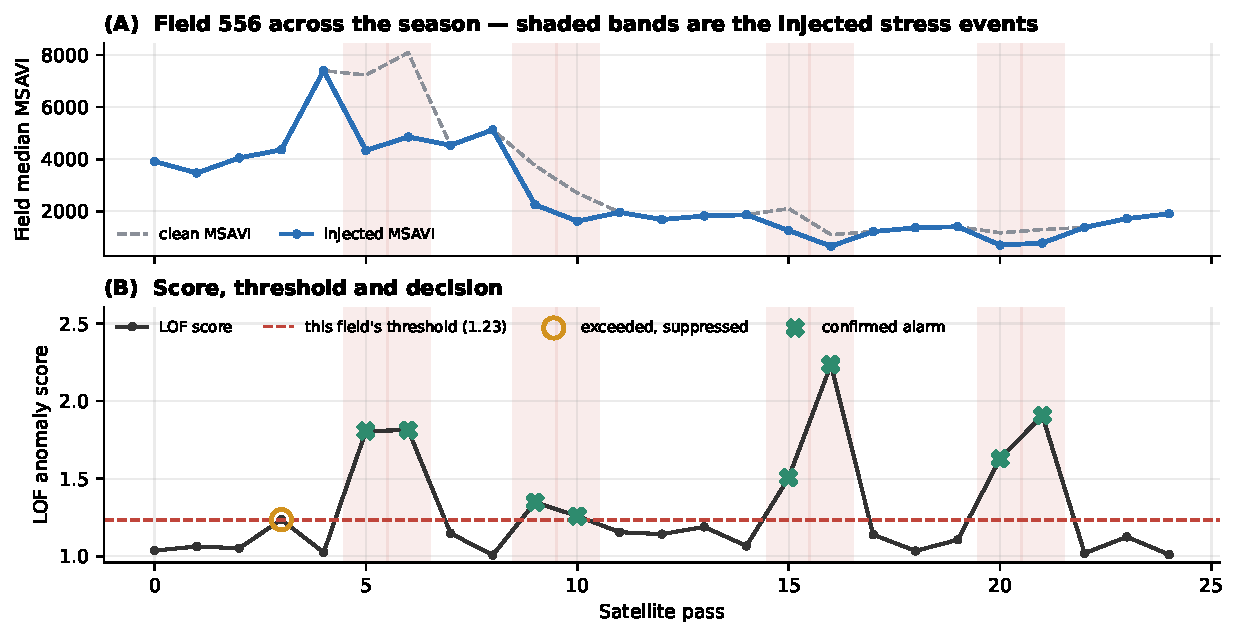
\includegraphics[width=0.80\textwidth]{worked_example.pdf}
\caption{One held-out tile, start to finish. \textbf{(A)} Tile median MSAVI,
clean and injected; shaded bands are the injected events. \textbf{(B)} LOF
score, the tile's own threshold, exceedances suppressed by the persistence rule
(open circles) and confirmed alarms (crosses). Of eight injected observations
the detector confirmed all eight with no false alarms, and suppressed one
isolated exceedance elsewhere in the season. That suppression is the cost of the
persistence requirement: the mechanism that removes transient cloud artefacts
also removes genuine one-pass events, and every recall figure in this paper is
net of it. Discussed in Section~\ref{sec:example}.}
\label{fig:example}
\end{figure*}

\subsection{Ensembling is harmful}
\label{sec:models}

\begin{table}[!t]
\caption{Detector comparison. All at the same operating point on the same
held-out tiles; each detector receives its own clean-data threshold, since the
three score scales are not comparable. Mean\,$\pm$\,s.d.\ over 5 seeds.}
\label{tab:models}
\centering
\tabfont
\begin{tabular}{lccccr}
\toprule
Detector & Prec. & Recall & F1 & PR-AUC & FA \\
\midrule
Isolation Forest   & 0.661 & 0.104 & 0.179 & 0.200 & 161 \\
\textbf{LOF}       & \textbf{0.876} & \textbf{0.814} & \textbf{0.844} & \textbf{0.904} & 350 \\
Autoencoder        & 0.848 & 0.383 & 0.528 & 0.487 & 209 \\
ISO + LOF          & 0.771 & 0.230 & 0.354 & 0.294 & 208 \\
Hybrid (all three) & 0.772 & 0.230 & 0.354 & 0.294 & 207 \\
\bottomrule
\end{tabular}
\end{table}

\begin{figure}[!t]
\centering
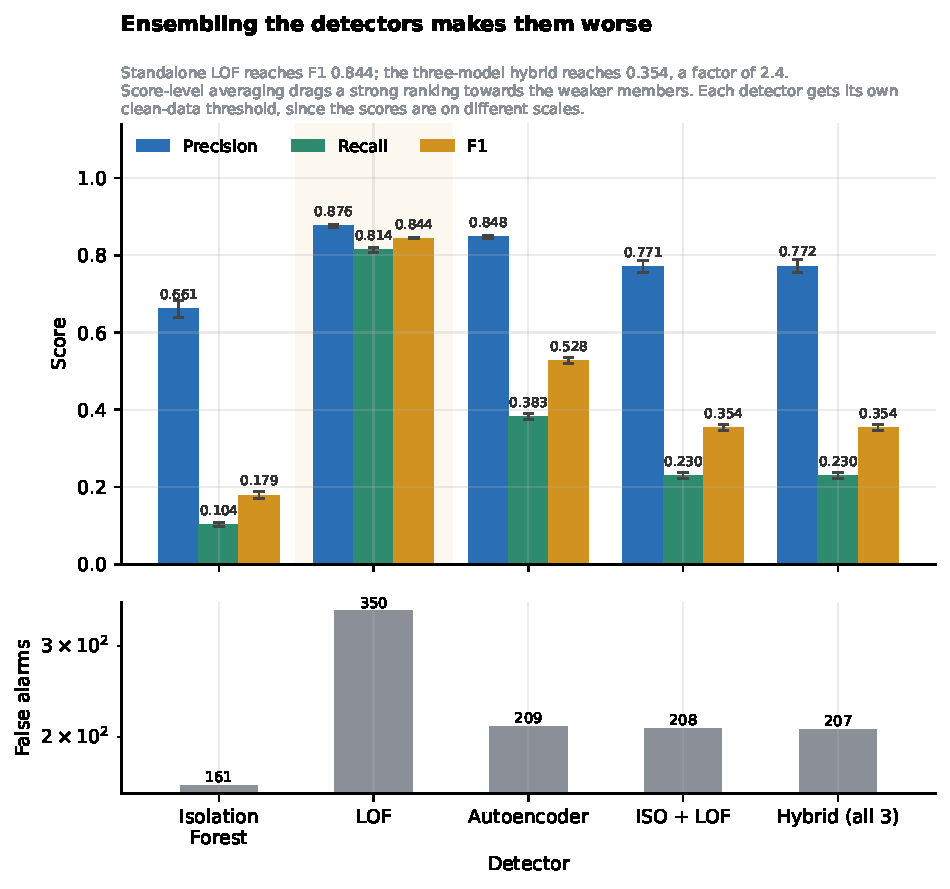
\includegraphics[width=\columnwidth]{detectors.pdf}
\caption{Ensembling degrades the detector it is meant to strengthen. The failure
is in recall, not precision: the ensembles still alarm accurately when they
alarm, but they stop alarming.}
\label{fig:models}
\end{figure}

Table~\ref{tab:models} and Fig.~\ref{fig:models} give the result, and it is the
opposite of what the system was built to demonstrate. Standalone LOF reaches F1
$0.844$; the three-model hybrid reaches $0.354$. Adding the autoencoder to
ISO+LOF changes nothing measurable, which tells us the ensemble score is
dominated by Isolation Forest.

The mechanism is visible in the columns. The ensembles retain respectable
precision ($0.77$) but collapse in recall, $0.814 \rightarrow 0.230$. Averaging
does not make the alarms wrong; it makes the detector quiet. A weighted sum of
normalised scores is only as discriminative as its components allow, so
averaging a ranking with PR-AUC $0.904$ against one at $0.200$ produces a
ranking closer to the weaker, and a per-tile threshold acting on that ranking
inherits the damage: genuinely stressed observations no longer sit in their
tile's upper tail.

Ensembling helps when members are individually competent and make
\emph{decorrelated} errors. Here they are not competent. Isolation Forest's
axis-aligned splits detect globally extreme feature values, but a stressed
observation of an intrinsically low-vigour tile is not a global extreme ---
precisely the case LOF's local density comparison is built for, and precisely
the case a large benchmark study identifies LOF as the right tool for
\cite{han2022}. We had a grid search over ensemble weights available and did not
pursue it: the correct weight vector is $(0,1,0)$, and tuning towards that
conclusion while still presenting the architecture as a hybrid would
misrepresent the data.

\subsection{Against rules written by hand}

\begin{table}[!t]
\caption{Learned detector versus rule-based scorers. Identical data, identical
threshold source and persistence rule; only the scoring function differs.}
\label{tab:baselines}
\centering
\tabfont
\begin{tabular}{lccccr}
\toprule
Method & Prec. & Recall & F1 & PR-AUC & FA \\
\midrule
\textbf{LOF (this work)} & \textbf{0.876} & \textbf{0.814} & \textbf{0.844} & \textbf{0.904} & 350 \\
Per-tile z-score         & 0.707 & 0.147 & 0.243 & 0.328 & 185 \\
Fixed \% drop            & 0.633 & 0.131 & 0.217 & 0.286 & 232 \\
Rolling-median deviation & 0.406 & 0.007 & 0.013 & 0.214 & \phantom{0}29 \\
\bottomrule
\end{tabular}
\end{table}

A learned detector should be shown to beat a rule that could have been written
without one. Table~\ref{tab:baselines} compares LOF against three rule-based
scorers, every one passing through an identical clean-calibrated threshold and
persistence path. LOF reaches F1 $0.844$ against $0.243$ for the strongest rule,
a $3.5\times$ margin, so the gain is attributable to the density-based scoring
rather than to the machinery around it.

\subsection{Where the threshold is computed}
\label{sec:threshold}

\begin{table}[!t]
\caption{Threshold rule. Same detector, same tiles, same injections, same
persistence rule --- only the threshold differs. The first row is the rule used
in an earlier version of this system.}
\label{tab:threshold}
\centering
\tabfont
\begin{tabular}{lcccr}
\toprule
Threshold rule & Prec. & Recall & F1 & FA \\
\midrule
Adaptive P85, post-injection & 0.825 & 0.597 & 0.693 & 384 \\
Global P90, post-injection   & \textbf{0.979} & 0.520 & 0.679 & \textbf{34} \\
Clean-calibrated P97.25      & 0.857 & \textbf{0.834} & \textbf{0.845} & 421 \\
\textbf{EVT / GPD ($q=0.03$)} & 0.876 & 0.814 & 0.844 & 350 \\
\bottomrule
\end{tabular}
\end{table}

\begin{figure}[!t]
\centering
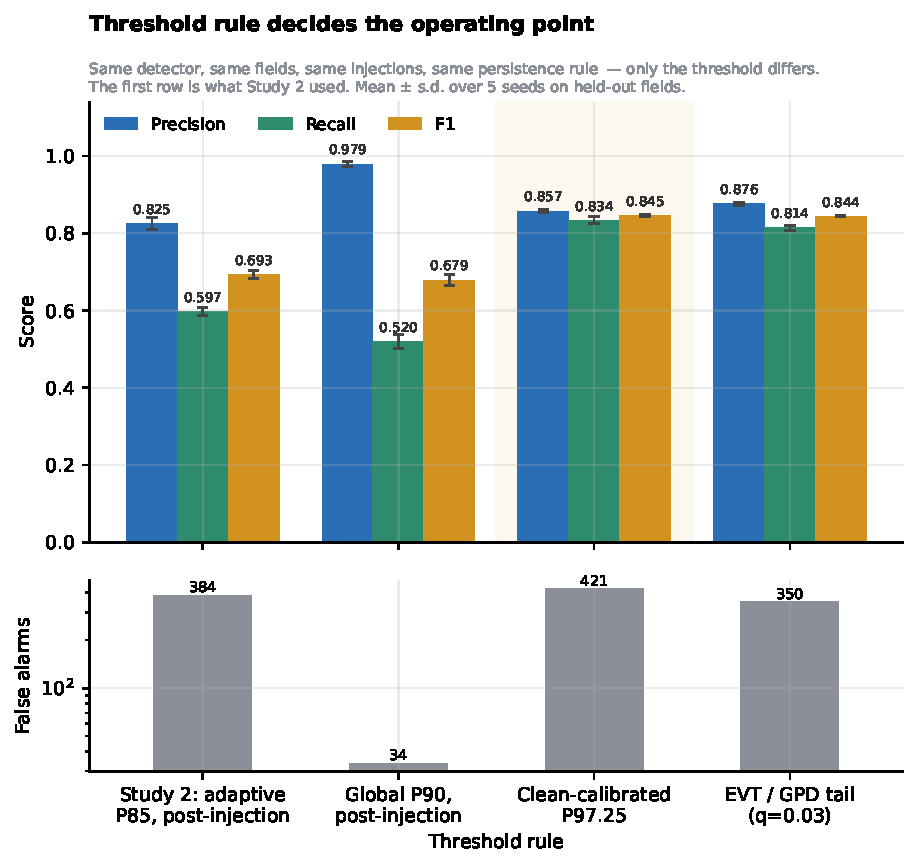
\includegraphics[width=\columnwidth]{threshold_rules.pdf}
\caption{The threshold rule, not the detector, sets the operating point. All
four rows use the same LOF scores on the same held-out tiles.}
\label{fig:threshold}
\end{figure}

Table~\ref{tab:threshold} and Fig.~\ref{fig:threshold} give the most
consequential result in the paper, and the one we did not expect.

Computing each tile's percentile on the batch that already contains the
injections is conventional in fully unsupervised work, where no clean
calibration set is assumed to exist. At a $15\%$ injection rate it is also a
specific trap. The top $15\%$ of scores \emph{are} the anomalies, so a P85 cut
lands exactly on their boundary and is dragged upward into the group it is meant
to separate. Roughly half the injected observations end up below their own
tile's threshold. This caps recall near $0.6$ regardless of which detector is
used --- which, in hindsight, explains a ceiling we had previously attributed to
the detector.

Calibrating the same threshold on clean, pre-injection scores removes the cap.
The percentile can then be set far stricter (P97.25, chosen on the calibration
tiles) and still recover more: F1 $0.693 \rightarrow 0.845$, recall
$0.597 \rightarrow 0.834$. Bootstrapping over $4{,}160$ tile-seed units gives
$\Delta$F1 $= +0.151$ with 95\% CI $[+0.142, +0.159]$ and paired permutation
$p < 5 \times 10^{-4}$ (no permutation of $2{,}000$ reached the observed
difference, so this is the resolution limit of the test rather than a point
estimate).

\textbf{An extreme-value alternative.} With $25$ observations per tile an
empirical percentile saturates: above roughly P96 it interpolates between the
top one or two scores, and no observation can exceed its own tile's threshold
at all. Following Siffer et al.\ \cite{siffer2017} we instead fit a Generalised
Pareto tail \cite{pickands1975,balkema1974} to each tile's clean scores and
invert it for a target false-alarm risk $q$. With only about five excesses per
tile the shape parameter is fitted once on pooled, scale-normalised excesses
($\xi = -0.199$, a bounded tail, as LOF scores on a homogeneous population
should give) and only the scale varies per tile.

At $q = 0.03$, chosen on the calibration tiles, this attains F1 $0.844$ with
$350$ false alarms against $421$ for the tuned percentile --- statistically
indistinguishable accuracy with $17\%$ fewer unnecessary inspections. Its real
advantage is expressive: it replaces \emph{we chose the 85th percentile} with
\emph{we chose a 3\% false-alarm risk}, which is a quantity a grower can be
asked about. We report it as the recommended configuration. Note that it was
selected on the calibration tiles and is narrowly \emph{behind} the percentile
rule on test F1; selecting the percentile rule on that basis would be the same
error this section diagnoses.

Global P90 remains the precision extreme: $0.979$ precision with $34$ false
alarms at $0.520$ recall. Where an unnecessary field visit is expensive
relative to a missed event, it is still the rule to deploy.

% Also declared ahead of its discussion (Sec. V-G), so it is not queued behind
% the full-width float above.
\begin{figure}[!tb]
\centering
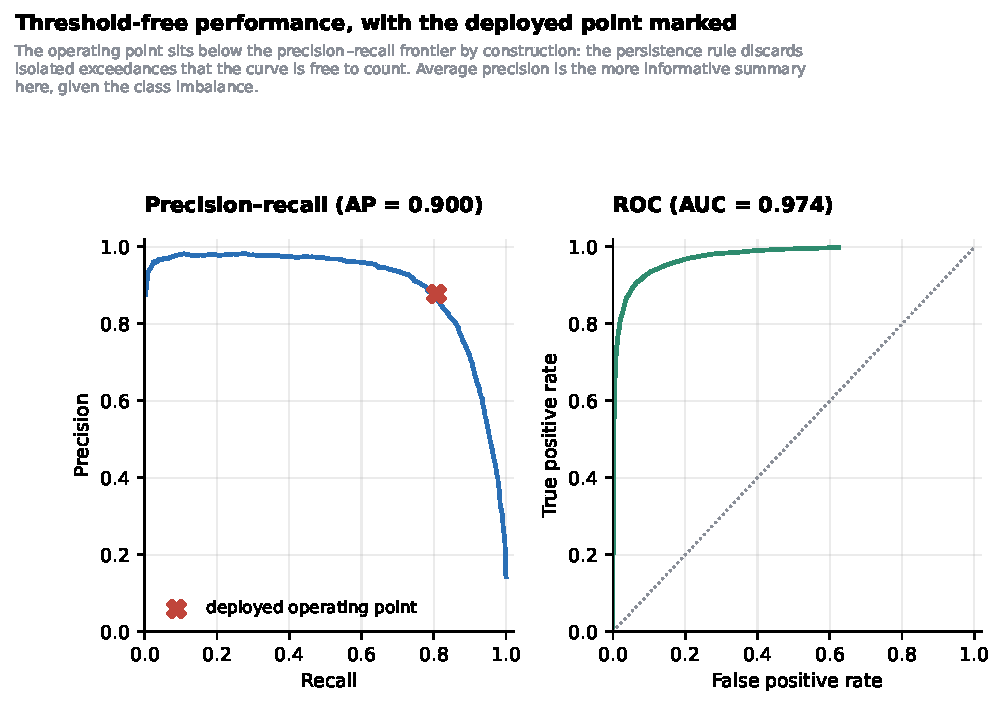
\includegraphics[width=\columnwidth]{curves.pdf}
\caption{Precision--recall and ROC characteristics of the LOF score, with the
deployed operating point marked. The point sits below the frontier by
construction, because the persistence rule discards isolated exceedances the
curve is free to count.}
\label{fig:curves}
\end{figure}

\subsection{Detection limits, and where this is worse}
\label{sec:limits}

\begin{table}[!t]
\caption{Detection limits. F1 by severity and duration. Severities below $30\%$
were evaluated only at $d=2$.}
\label{tab:limits}
\centering
\tabfont
\begin{tabular}{lccccc}
\toprule
Duration & 10\% & 20\% & 30\% & 40\% & 50\% \\
\midrule
$d=1$ & --- & --- & 0.365 & 0.452 & 0.500 \\
$d=2$ & 0.077 & 0.482 & 0.755 & 0.844 & 0.859 \\
$d=3$ & --- & --- & 0.786 & 0.877 & \textbf{0.898} \\
\bottomrule
\end{tabular}
\end{table}

\begin{figure}[!t]
\centering
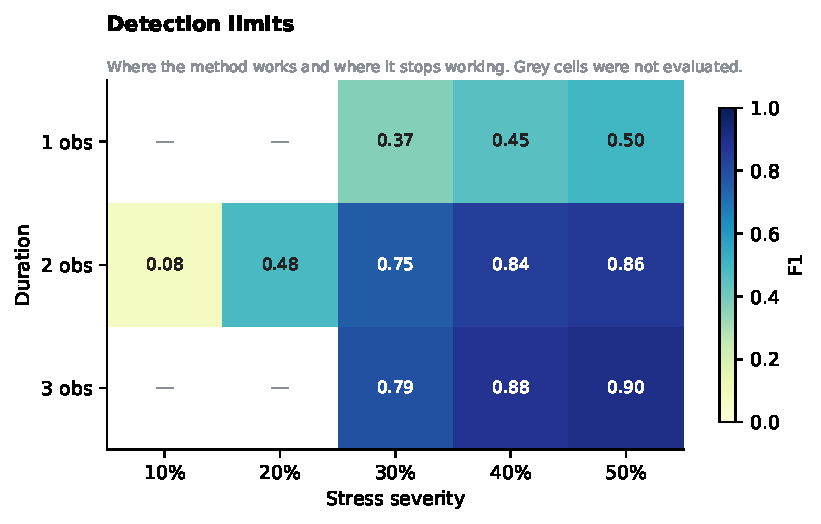
\includegraphics[width=\columnwidth]{limits.pdf}
\caption{Detection limits. The method is reliable for events of at least
$30\%$ severity persisting two or more passes, and fails on weak or
single-pass events.}
\label{fig:limits}
\end{figure}

Table~\ref{tab:limits} and Fig.~\ref{fig:limits} bound what the method can see.
Detection is reliable
above $30\%$ severity for two or more passes. Two failure regions are
structural: a $10\%$ depression of a tile-mean index is comparable to the
pass-to-pass variation the index shows anyway under changing illumination, and
single-pass events are suppressed by design, since the persistence rule cannot
distinguish a one-pass excursion from a cloud artefact on temporal evidence
alone.

\textbf{The recommended operating point is not uniformly better.} Against the
adaptive-P85 rule it replaces, it wins on nine of eleven severity--duration
cells, often by more than $0.12$~F1 --- but it \emph{loses} on the two weakest:
F1 falls $0.546 \rightarrow 0.482$ at $20\%$ severity and $0.233 \rightarrow
0.077$ at $10\%$. The risk $q$ was chosen at $40\%$ severity, so the threshold
sits high enough that a shallow dip barely clears it and recall collapses.

We state this prominently because it inverts the recommendation for one
important use case. If the goal is early warning of \emph{developing} stress,
a looser threshold is correct and the headline numbers here are the wrong ones
to quote. If the goal is reliable detection of established stress with few false
alarms, this operating point is correct. The honest reading is that $q$ is a
dial set from the relative cost of a missed event and a wasted field visit, and
that a single operating point should not be reported as though it were optimal
for all of them.

\subsection{Where the false alarms fall}
\label{sec:alarmmap}

\begin{figure}[!t]
\centering
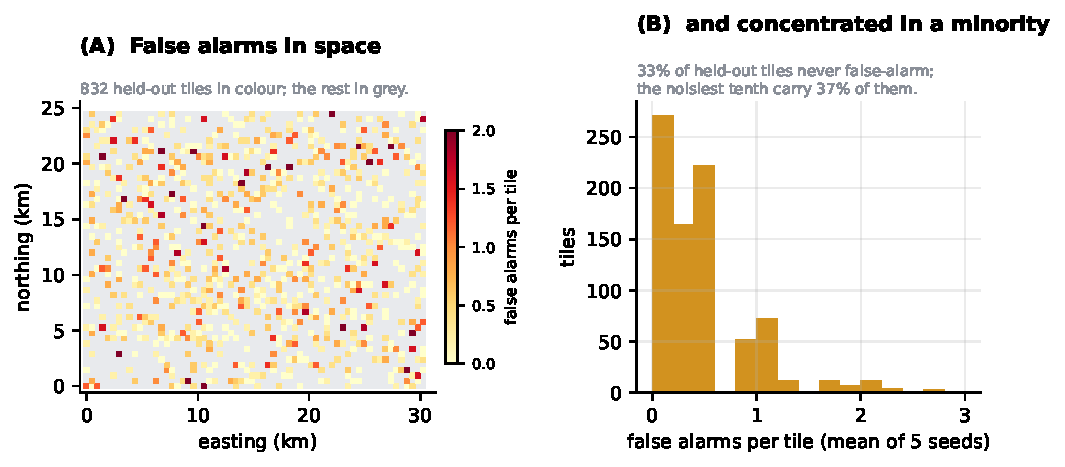
\includegraphics[width=\columnwidth]{alarm_map.pdf}
\caption{\textbf{(A)} The $350$ false alarms placed on the ground: held-out
tiles coloured by their mean false-alarm count over the five seeds, the
remaining tiles in grey. \textbf{(B)} The same counts as a distribution. False
alarms are not spread evenly and do not form geographic clusters; they
concentrate on individual tiles.}
\label{fig:alarmmap}
\end{figure}

Every table above reports false alarms as a single count. Because each tile is
georeferenced we can ask a question the count hides: are those $350$ alarms
spread thinly across the region, or carried by a few bad tiles?
Fig.~\ref{fig:alarmmap} answers it. Roughly a third of held-out tiles never
false-alarm at all across five seeds, while the noisiest tenth account for
about $37\%$ of the total. The pattern is not geographic --- no cluster, no
edge effect --- so it is not weather or a processing artefact over part of the
scene. It is a property of individual tiles, which is what a per-tile threshold
would be expected to leave behind: the threshold normalises for how variable a
tile is on clean data, but a tile whose clean scores are heavy-tailed still
crosses its own cut more often than a well-behaved one.

This has an operational consequence the aggregate number obscures. A deployed
system does not have to accept a uniform inspection burden; a tile that alarms
repeatedly without a corresponding event is a candidate for a watchlist, a
raised threshold, or exclusion pending a crop-type check. We do not implement
that here --- it would be tuning against our own injections --- but the
concentration is strong enough that it is the first thing we would try, and it
is only visible because the unit of analysis carries a location.

\subsection{Persistence and stress signature}

\begin{table}[!t]
\caption{Persistence rule, at 2-observation events. All four rules are causal.}
\label{tab:persistence}
\centering
\tabfont
\begin{tabular}{lcccr}
\toprule
Rule & Prec. & Recall & F1 & FA \\
\midrule
None                      & 0.755 & \textbf{0.870} & 0.809 & 859 \\
\textbf{Strict 2-consec.} & \textbf{0.876} & 0.814 & \textbf{0.844} & 350 \\
Sliding 2-of-3            & 0.534 & 0.525 & 0.530 & 1{,}388 \\
Strict 3-consec.          & 0.762 & 0.335 & 0.465 & \textbf{317} \\
\bottomrule
\end{tabular}
\end{table}

Persistence trades recall for precision (Table~\ref{tab:persistence}). Strict
$2$-consecutive is our default. Two remarks are needed to read the table
correctly. The sliding $2$-of-$3$ window scores below no persistence at all:
relaxing consecutiveness admits scattered isolated exceedances faster than it
recovers genuine events. And the $3$-consecutive row is measured at
$2$-observation events, so the rule cannot fire on the event alone --- its low
score there is a consequence of the scenario, not evidence about the rule. All
four rules are causal, inspecting only $[t-2, t-1, t]$.

\begin{table}[!t]
\caption{Robustness to the stress signature, at the recommended operating point.}
\label{tab:types}
\centering
\tabfont
\begin{tabular}{lccccr}
\toprule
Signature & Prec. & Recall & F1 & PR-AUC & FA \\
\midrule
Sudden drop    & 0.876 & 0.814 & \textbf{0.844} & 0.904 & 350 \\
Spectral shift & 0.868 & 0.757 & 0.809 & 0.854 & 349 \\
Gradual onset  & 0.872 & 0.474 & 0.614 & 0.745 & 211 \\
\bottomrule
\end{tabular}
\end{table}

Against the three signatures (Table~\ref{tab:types}) the pipeline handles abrupt
declines and spectral shifts comparably but is markedly weaker on gradual onset
(F1 $0.614$). The cause is the rolling baseline: a slowly accumulating decline
is partly absorbed into the rolling median the features are computed against, so
the tile's own reference drifts down with the stress and the residual stays
small. This is the agronomically inconvenient failure, since progressive drought
and spreading foliar disease --- where early warning is worth most --- are
exactly slow-onset events.

\subsection{A worked example}
\label{sec:example}

Fig.~\ref{fig:example} traces the full decision path on one tile. It also shows
what the rule discards: an isolated exceedance that crossed the tile's own
threshold, did not recur, and was therefore dropped.

\subsection{Threshold-free performance}

Every table above is measured at one operating point, which leaves open whether
the ranking is good or the cut merely lucky. Average precision is $0.900$ and
ROC-AUC $0.974$ (Fig.~\ref{fig:curves}), both threshold-free; average precision
is the more informative under this class balance.

%=======================================================================
\section{What Held-Out Evaluation Costs}
\label{sec:protocol}

\begin{table}[!t]
\caption{Protocol effect. Only the set of tiles the detector is fitted on
changes; the threshold rule, features and injections are identical.}
\label{tab:protocol}
\centering
\tabfont
\begin{tabular}{lcccr}
\toprule
Protocol & Prec. & Recall & F1 & PR-AUC \\
\midrule
Same tiles (fitted on all)      & 0.836 & 0.623 & 0.714 & 0.945 \\
Held-out (disjoint half)        & 0.825 & 0.597 & 0.693 & 0.904 \\
\bottomrule
\end{tabular}
\end{table}

Fitting LOF in novelty mode on the same tile-seasons it later scores is
conventional, and the fit precedes injection so no anomaly is seen --- but the
\emph{tiles} are not held out. Campos et al.\ \cite{campos2016} give good
reason to expect such choices to matter.

An earlier version of this work compared its numbers against an independent
re-implementation evaluated on held-out tiles, observed F1 $0.72$ against
$0.35$, and read the gap as an evaluation-protocol effect. That comparison was
uncontrolled: the two implementations also differed in input representation,
cloud screening, observation density and injection procedure.

Table~\ref{tab:protocol} isolates the protocol. Holding everything else fixed,
fitting on a disjoint half of the tiles costs $0.021$~F1. \textbf{The protocol
does not account for the gap.} Whatever separates those two numbers lives in the
other differences, and we withdraw the earlier attribution. We report this
because a plausible-sounding effect measured across two codebases survived
internal review in our own project until it was tested directly, which is
exactly the failure mode \cite{campos2016} warns about.

%=======================================================================
\section{Discussion and Limitations}
\label{sec:forward}

\textbf{Synthetic injection is a proxy, and a generous one.} Every number here
rests on injected anomalies, and the mechanism deserves scrutiny. Injection
scales six of the sixteen features by $(1-\text{severity})$ and the derived
temporal features inherit the perturbation, so a simulated event is a large,
coherent displacement \emph{in exactly the space the detector operates in}. Real
stress is spatially heterogeneous within a tile, partial, and confounded with
phenological stage. The absolute figures should therefore be read as an upper
bound, and the comparisons \emph{between} configurations --- which is what the
ablations measure --- as the reliable part. Validation against a ground-truth
campaign, even a small one, remains the most valuable missing evidence and
nothing here substitutes for it.

\textbf{The method is weakest where it would be most valuable.} The headline
scenario is a $40\%$ decline over two passes, which a grower would likely notice
unaided. At $10$--$20\%$ severity F1 is $0.08$--$0.48$
(Section~\ref{sec:limits}), and gradual onset scores $0.614$ against $0.844$ for
an abrupt drop. Early detection of developing stress is the application that
justifies the work, and it is the regime the method handles least well.

\textbf{Clean calibration assumes a stress-free reference period.} Within a
retrospective seasonal analysis that is available. For a real-time system it is
an assumption, and the obvious source --- the previous season --- is unreliable:
in a separate study we found that using a field's prior season as its baseline
performed \emph{worse} than using other fields in the current season, because
crop rotation gives a field a different normal from one year to the next. A
deployed system would need crop-type conditioning or a within-season peer group.

\textbf{Scope.} One region, one season, one crop mix, one cloud regime. We have
not tested transfer. The test split is $832$ tiles, so these figures carry more
sampling noise than a whole-dataset number.

\textbf{The split is disjoint in tiles but not in space.} Tiles are assigned to
fit, calibration and test at random over their identifiers, which leaves the
three sets spatially interleaved: $94\%$ of held-out tiles share an edge with a
tile the detector was fitted on (Fig.~\ref{fig:studyarea}B). Adjacent tiles in a
$480$\,m grid over one irrigated plain share weather, haze, soil and often crop
and management, so held-out tiles are less independent of the fitted ones than
the term suggests. This is the failure mode that spatially blocked
cross-validation exists to avoid: random splits over autocorrelated data
systematically overstate predictive performance, and the effect is large enough
in ecological mapping to reverse published conclusions
\cite{roberts2017,ploton2020}. Two consequences follow. Our headline numbers may
be optimistic relative to a deployment in an unseen region, and --- more
specifically --- the $0.021$~F1 cost of held-out evaluation reported in
Section~\ref{sec:protocol} is measured under exactly this interleaving, so it
should be read as a lower bound on what a spatially blocked split would cost.
Testing that properly requires re-running the protocol with contiguous spatial
blocks held out, which we have not done; we flag it as the most important
untested assumption in the evaluation.

\textbf{Statistical strength.} Reported spreads are across five injection seeds
and capture injection variance only, not variation across regions, seasons or
tile populations. The bootstrap in Section~\ref{sec:threshold} resamples
tiles and is the stronger test.

\textbf{Tile-level only.} The detector emits one score per tile per pass and
does not localise within a tile.

\textbf{The clearest route forward} is spectral rather than algorithmic. The raw
archive is nine-band, so NDVI, NDRE and NDMI are computable alongside MSAVI; in a
separate study, deriving four indices instead of one raised F1 by $44\%$
relative under a matched protocol. NDMI responds to canopy water content rather
than chlorophyll and correlates only $0.81$--$0.85$ with the greenness indices,
so it carries independent signal. Since water stress precedes visible greenness
loss, this is also the most promising attack on the gradual-onset weakness ---
the failure mode that currently matters most.

%=======================================================================
\section{Conclusion}

We presented a fully unsupervised tile-level crop stress detector for
Sentinel-2 time series, evaluated with no labels at any stage on held-out tiles
under a protocol in which nothing reported is selected on. LOF with an
extreme-value threshold and a strict two-consecutive persistence rule reaches
precision $0.876$, recall $0.814$ and F1 $0.844$ against injected $40\%$
two-pass events.

The two findings we expect to outlast that number are not about the number.
Score-level ensembling of Isolation Forest, LOF and an autoencoder is not a
robustness improvement but a collapse in recall, from $0.814$ to $0.230$,
because averaging a strong ranking with weak ones destroys the ranking that the
per-tile threshold then acts on. And \emph{where} the threshold is computed
matters more than \emph{which} detector produces the score: moving the
calibration from the injected batch to clean data improved F1 by $0.151$ with
the detector untouched, an effect larger than the difference between most
detectors we tested.

We also withdraw a claim from our own earlier work. A large apparent cost of
held-out evaluation, obtained by comparing two implementations, does not survive
a controlled test; the true cost is $0.021$~F1. We report the correction because
the original claim was plausible, internally reviewed, and wrong.

%=======================================================================
\section*{Reproducibility}

All experiments are deterministic given the five reported seeds. Figures,
tables and the results document are regenerated by a single script from one
stored results file, so plotted and reported numbers cannot diverge.

%=======================================================================
\bibliographystyle{IEEEtran}
\bibliography{refs}

\end{document}
